\chapter{Eccezioni}

\section{Definizione}
Un eccezione è un evento \textbf{sincrono}, generato all'interno del processore e provocato da problemi nell'esecuzione di un'istruzione

\subsection{Esempi di eccezioni}
\begin{itemize}
    \item Overflow
    \item Istruzione non valida
    \item Errori
    \item Pagine non presenti
    \item \dots
\end{itemize}

\section{Procedura generale per la gestione di un eccezione}

\subsection{Procedura generale}
\begin{enumerate}
    \item Interruzione dell'esecuzione del programma corrente
    \item Salvataggio parziale dello stato di esecuzione corrente per riprendere eventualmente l'esecuzione del programma corrente se possibile
    \item Salto a una routine del sistema operativo per gestire l'eccezione (tale routine è chiama di solito exception handler)
    \item Esecuzione della routine del SO
    \item Se possibile, ripristino dello stato di esecuzione del programma e continuazione dell'esecuzione del programma
\end{enumerate}

\subsection{Problematica: Identificazione dell'evento inatteso}
Per capire quale sia l'evento inatteso verificatosi si hanno 2 possibili soluzioni

\subsubsection{Indirizzo fisso}
Il controllo della CPU, prima di saltare all'handler del SO (a un indirizzo fisso), deve saltare in un registro interno un identificatore numerico del tipo di eccezione verificatosi.

L'handler accederà al registro interno per determinare la causa dell'eccezione

\subsubsection{Interruzioni vettorizzate}
Il controllo della CPU sceglie l'handler corretto, saltando all'indirizzo corretto.

A questo scopo, viene predisposto un vettore di indirizzi, uno per ogni tipo di eccezione, da indirizzare tramite il codice numerico dell'eccezione

\vspace{0.3cm}

\begin{center}
    \begin{tabular}{|c|c|}
        \hline \textbf{Tipo di eccezione} & \textbf{Exception vector address (in hex)} \\ \hline

        Undefined Instruction & $\texttt{C000\ 0000}_{hex}$ \\ \hline

        Arithmetic Overflow & $\texttt{C000\ 0020}_{hex}$ \\ \hline
        
    \end{tabular}
\end{center}

\section{Gestione delle eccezioni in MIPS}

\subsection{Registri Coprocessore 0}
Nel MIPS viene adottata la prima soluzione

\begin{itemize}
    \item Il registro \textbf{Cause} viene usato per memorizzare il motivo dell'eccezione
    
        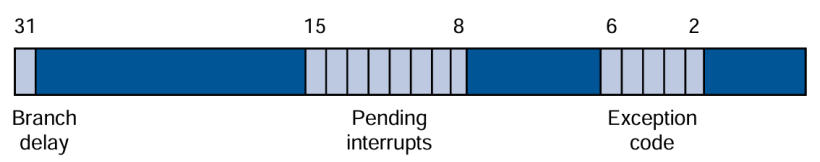
\includegraphics[scale=0.5]{Immagini/Registro cause.png}

    \item Il registro \textbf{EPC - Exception Program Counter} viene usato per memorizzare l'indirizzo dell'istruzione corrente che ha causato l'eccezione 
    \item Il registro \textbf{Status} viene usato per memorizzare la maschera delle interruzioni e bit di abilitazione
    
        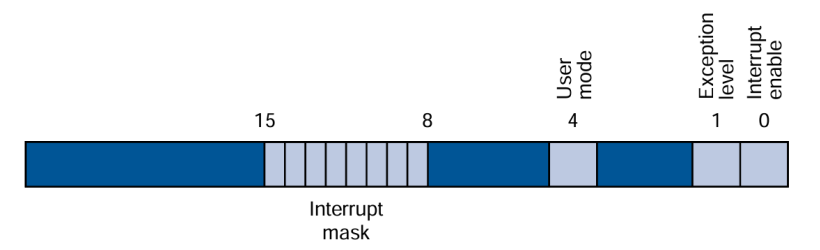
\includegraphics[scale=0.5]{Immagini/Registro Status.png}

    \item Il registro \textbf{BadVAddr} viene usato per memorizzare l'indirizzo di memoria il cui riferimento ha provocato l'eccezione
\end{itemize}

\subsection{Procedura}
    \subsubsection{Azioni a carico dell'hardware}
    \begin{enumerate}
        \item Individuare l'evento inatteso, la causa dell'eccezione e salvarla all'interno del registro Cause
        \item Interrompere l'esecuzione corrente
        \item Salvare l'indirizzo dell'istruzione corrente nel EPC ($EPC = PC-4$)
        \item Saltare all'indirizzo dell'exception handler
    \end{enumerate}

    \subsubsection{Azioni a carico dell'exception handler}
    \begin{enumerate}
        \item [4.] L'Exception Handler salva in memoria lo stato dei registri general purpose che intende utilizzare durante l'elaborazione, ad eccezione dei registri riservati $k0 e $k1. Non si salvano i registri del coprocessore, semmai se ne legge il contenuto.
        \item [5.] Gestisce l'eccezione, dopodiché ripristina dalla memoria i registri general purpose salvati in precedenza ed esegue l'istruzione eret per ritornare al programma originale, riprendendo l'esecuzione dall'indirizzo specificato da EPC
    \end{enumerate}


\subsection{Tabella delle eccezioni}
\begin{center}
    \begin{tabular}{|c|l|l|}
    \hline
    \textbf{Number} & \textbf{Name} & \textbf{Cause of exception} \\
    \hline
    0 & Int & interrupt (hardware) \\
    \hline
    4 & AdEL & address error exception (load or instruction fetch) \\
    \hline
    5 & AdES & address error exception (store) \\
    \hline
    6 & IBE & bus error on instruction fetch \\
    \hline
    7 & DBE & bus error on data load or store \\
    \hline
    8 & Sys & syscall exception \\
    \hline
    9 & Bp & breakpoint exception \\
    \hline
    10 & RI & reserved instruction exception \\
    \hline
    11 & CpU & coprocessor unimplemented \\
    \hline
    12 & Ov & arithmetic overflow exception \\
    \hline
    13 & Tr & trap \\
    \hline
    15 & FPE & floating point \\
    \hline
    \end{tabular}
\end{center}